The robot end effector is moved back and forth between two points along a diagonal in the robot workspace, see fig.~\ref{fig:path}. The trajectory is from XYZ (0.5,-0.5,0.45) to (0.25,0.6,-0.1) in meters and is repeated 9 times. Optitrack camera system is used to track the end effector. The test is performed at 30 mm/s and 50 mm/s on two different robots. Tests at 50 mm/s (above maximal nominal speed) show more vibration and better demonstrate the vibration damping from torque feedback.

\begin{figure}
	\begin{center}
	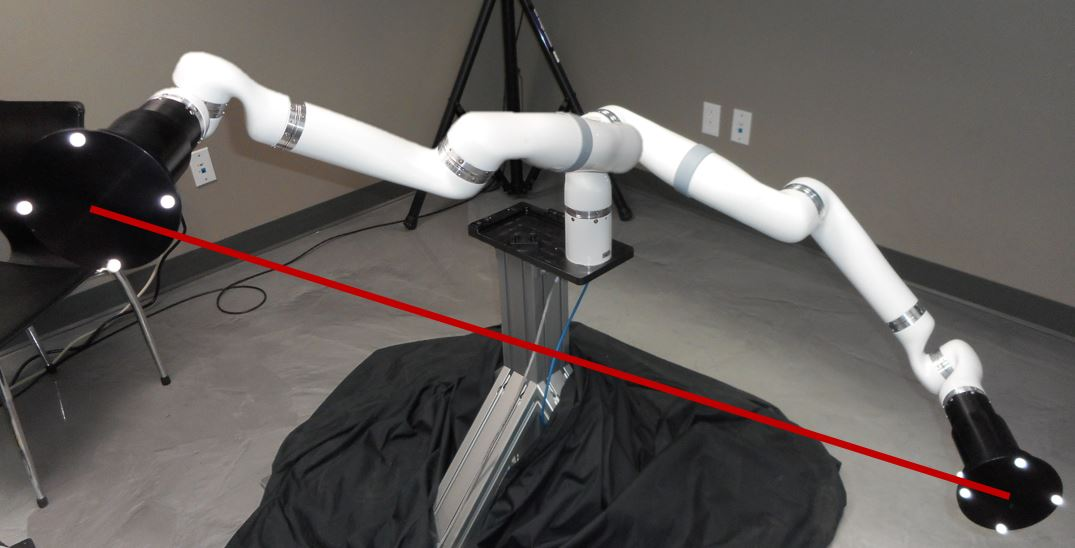
\includegraphics[width=.8\textwidth]{./images/testPath.jpg}%
		\caption{Test Trajectory}
	\label{fig:path}
	\end{center}
\end{figure}

From previous tests, vibration frequencies are known to be above 5~Hz. Therefore, a high-pass filter at 1~Hz is applied on the collected data to isolate vibration.  The mean, standard and maximum deviations are computed from it. Filtered data from two parts (over the 9) of the trajectory are shown in fig.~\ref{fig:data}. Regions of the trajectory showing worst behavior in terms of vibration are isolated and the same (but local) analysis is performed, see enclosed regions in fig.~\ref{fig:data}. All results are shown in table~\ref{table:results_torque}.

\begin{figure}
	\begin{center}
			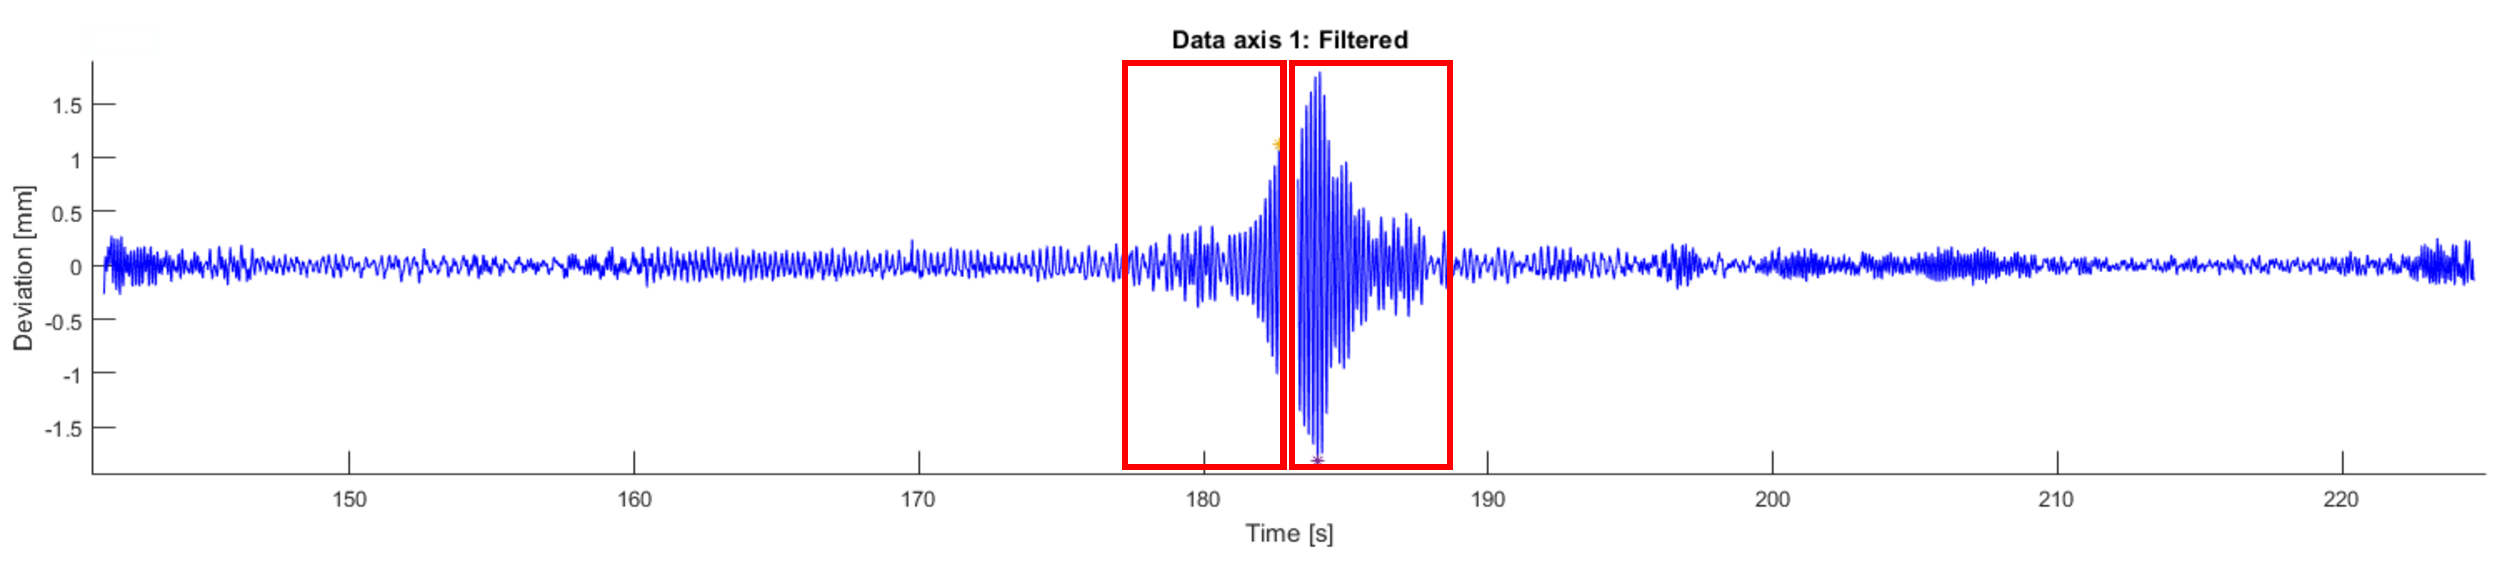
\includegraphics[width=1\textwidth]{./images/data2.pdf}%
			\caption{Filtered data from 2 parts of the trajectory and selected region for local analysis - Errata mm should be m}
			\label{fig:data}
	\end{center}
\end{figure}